\documentclass[cmpiitalkstyle, 25pt]{cmptalk}
\usepackage[utf8]{inputenc}

\hypersetup{pdfstartpage=1}%,pdfpagemode=FullScreen}%,pdfpagemode=None}
%\hypersetup{pdftitle=,pdfauthor=,pdfsubject=,pdfkeywords=}

\usepackage{bigfig,thumbpdf}
\usepackage[coloremph,display]{texpower}
%\usepackage[display]{texpower}
\usepackage{movie15}
%\usepackage{media9}

\newdimen\tmpd
\newbox\cmptalkverbbox

% notes customization (this one should be before begin document)
\cmptalkeverynotes={\usepackage{multicol}\usepackage{hyperref}\usepackage{movie15}}

\graphicspath{{../images/}}

%------------------------------------------------------------------- Title page
%-- specifications
\author{Pavel Trutman}
\affiliation{Centrum strojového vnímání}
\title{Generátor řešení minimálních problémů}
\acknowledgement{Vedoucí práce: Ing.\ Tomáš Pajdla, Ph.D.\\
Oponent: doc.\ Dr.\ Ing.\ Radim Šára}
\talklogo{\includegraphics[width=4cm]{cmp}}

\begin{document}
\bigfigfalse
\maketalktitlepage

% --------------------------------------------------------------------------- 
\begin{cmptalkslide}[Obsah]
  \begin{itemize}
    \item Motivace
    \item Automatický generátor
    \item Implementovaná vylepšení
    \end{itemize}
    \begin{narrow}[2]
    \begin{itemize}
      \item Víceeliminační postupy řešení
      \item Rozklad matic
      \item $F_4$ Algoritmus
    \end{itemize}
    \end{narrow}
    \begin{itemize}
    %\item Benchmark Automatického generátoru
    \item Experimenty
  \end{itemize}
\end{cmptalkslide}

% --------------------------------------------------------------------------- 
\begin{cmptalkslide}[Motivace]
  \begin{itemize}
    \item Mnoho problémů v počítačovém vidění vede na řešení soustav polynomiálních rovnic
    \item Tyto soustavy chceme umět řešit rychle $\rightarrow$ speciální postupy řešení
    \item Postupy řešení lze generovat automaticky $\rightarrow$ Automatický generátor \cite{AutoGen}
    \item Cílem je vylepšit Automatický generátor \cite{AutoGen}, aby generoval rychlejší a stabilnější postupy řešení
  \end{itemize}
\end{cmptalkslide}

% --------------------------------------------------------------------------- 
\begin{cmptalkslide}[Automatický generátor]
  \begin{itemize}
    \item Z parametricky zadaných polynomiálních rovnic generuje postupy řešení, které umožňují tyto soustavy řešit pro konkrétní parametry
    \item Původní implementace \cite{AutoGen} generuje jednoeliminační postupy řešení
    %\item Systematicky generuje polynomy vyšších stupňů, dokuď nejsou vygenerovány všechny potřebné polynomy k extrakci řešení pomocí vlastních čísel a vektorů
    %\item Gauss-Jordanova eliminace
    %\item Sestavení multiplikativní matice
    %\item Extrakce řešení z vlastních vektorů multiplikativní matice
  \end{itemize}

  \placeat{
    \Put(.5,0.3){\includegraphics[width=25cm]{AutomaticGenerator-presentation.pdf}}
  }

\end{cmptalkslide}

% --------------------------------------------------------------------------- 
\begin{cmptalkslide}[Víceeliminační postupy řešení]
  \begin{itemize}
    \item Polynomy generujeme systematicky, ale pravidelně je redukujeme pomocí Gauss-Jordanovy eliminace
    %\item Provedeme Gauss-Jordanovu eliminaci
    %\item Toto opakujeme dokud se generují nové polynomy
    %\item Zvýšíme stupeň generovaných polynomů o $d$
    \item Počet eliminací lze jednoduše řídit
    \item Víceeliminační postupy řešení jsou efektivní zvlášťe pro soustavy s velkým počtem neznámých
  \end{itemize}
\end{cmptalkslide}

% --------------------------------------------------------------------------- 
\begin{cmptalkslide}[Rozklad matic]
  \begin{itemize}
    \item Automatický generátor často pracuje s řídkými maticemi
    \item Snaha zrychlit Gauss-Jordanovu eliminaci řídkých matic
    \item Vycházeli jsme z poznatků \cite{SBBD}, že permutacemi sloupců a řádků lze matici převést do SBBD\footnote{Signly-bordered block-diagonal form} tvaru
    \item Poté lze provést dvě eliminace polovičních matic místo jedné eliminace celé matice
    \item Teoretické zrychlení je $n^3 \rightarrow 2\left(\frac{n}{2}\right)^3$
  \end{itemize}

  \placeat{
    \Put(.75,0.25){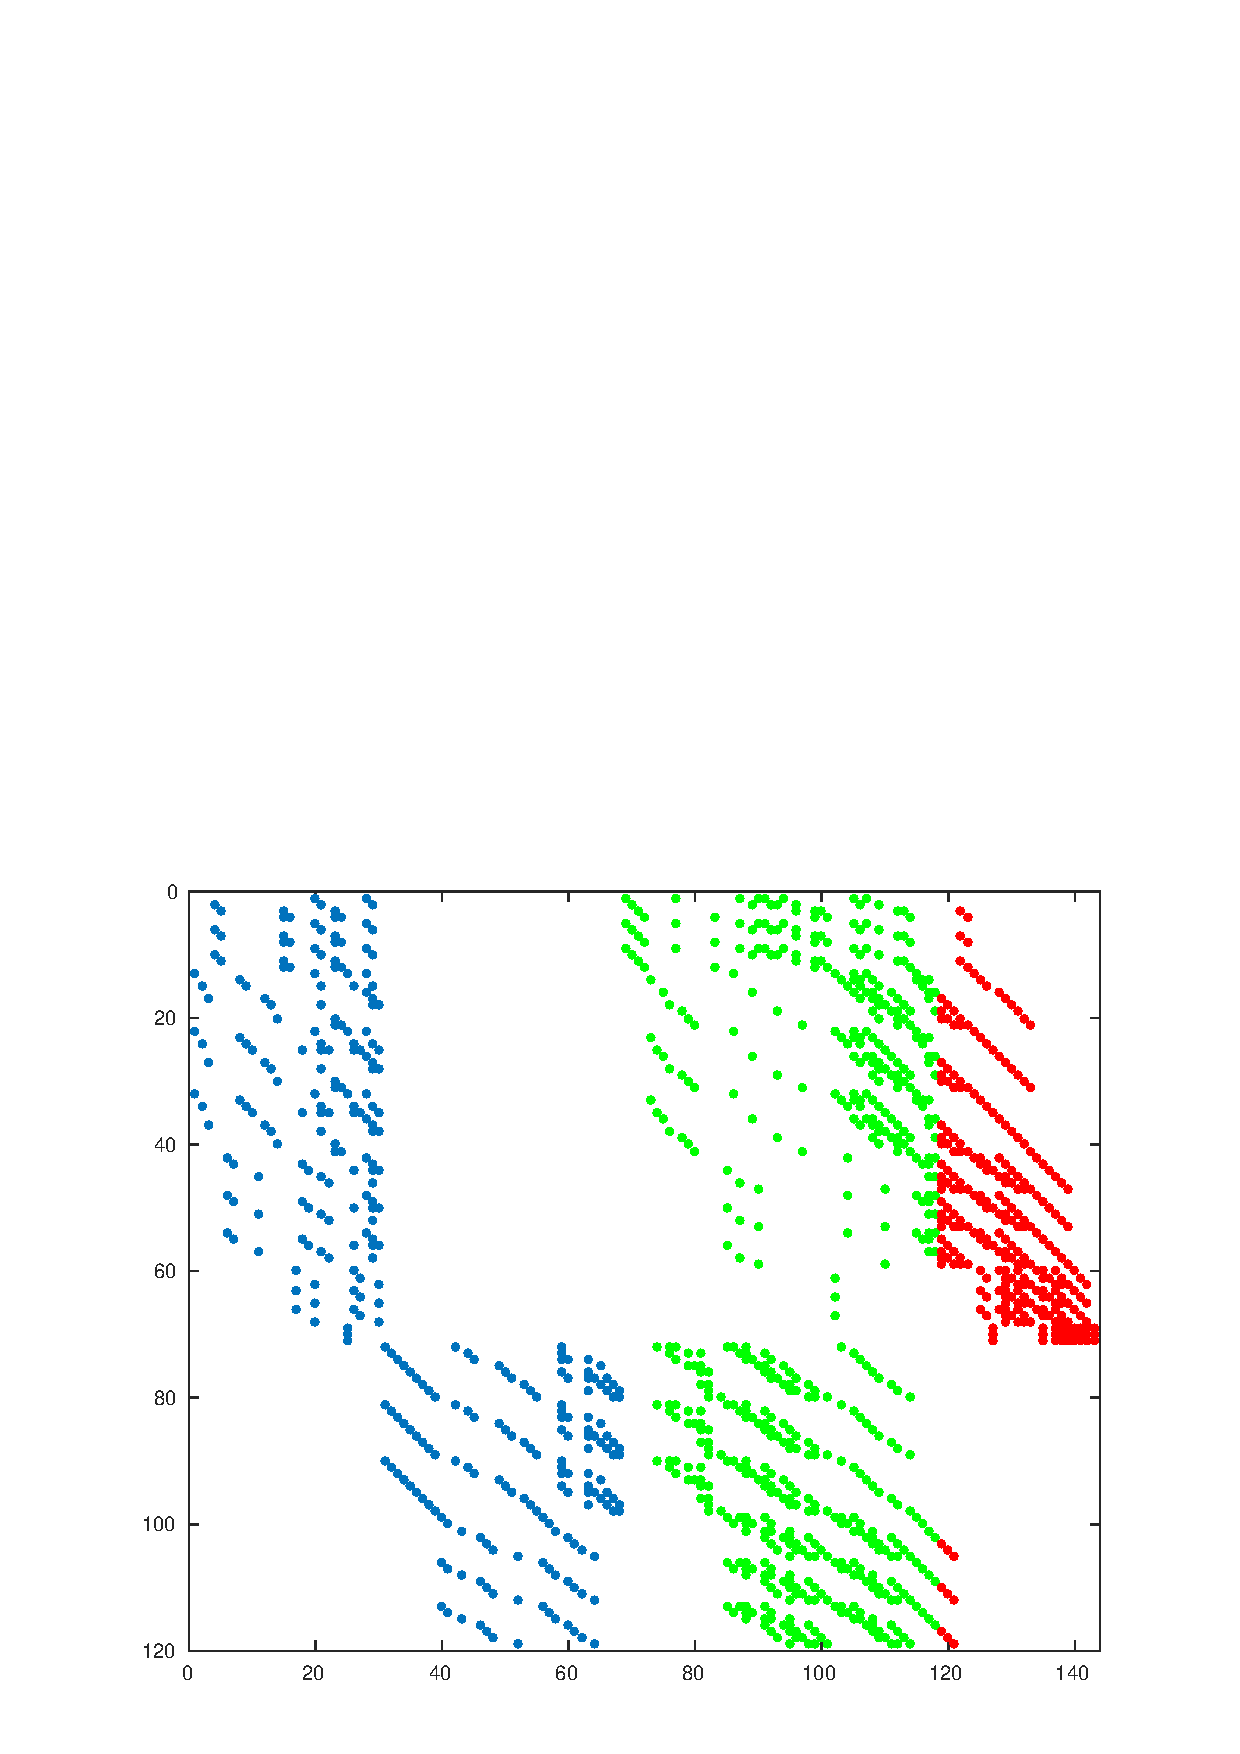
\includegraphics[width=14cm]{PaToH/permutation.pdf}}
  }
\end{cmptalkslide}

% --------------------------------------------------------------------------- 
\begin{cmptalkslide}[$F_4$ Algoritmus]
  \begin{itemize}
    \item $F_4$ Algortimus \cite{F4} konstruuje Gr\"obnerovu bázi systému polynomů
    \item Nejprve jsme algoritmus implementovali v Maple, abychom jemu porozuměli a ověřili funkčnost implementace
    \item $F_4$ Algoritmus jsme implementovali do Automatického generátoru \cite{AutoGen}
    \item Uživatel si může vybrat, zda se polynomy budou generovat systematicky nebo s využitím $F_4$ Algoritmu
  \end{itemize}
\end{cmptalkslide}

% --------------------------------------------------------------------------- 
%\begin{cmptalkslide}[Benchmark Automatického generátoru]
%  \begin{itemize}
%    \item Z vygenerovaných potupů řešení různými metodami je třeba vybrat ten nejvhodnější pro danou aplikaci
%    \item Uživatel si zvolí, které metody chce použít pro generování postupů
%    \item Zadá testovací data, případně jsou benchmarkem vygenerována náhodná data
%    \item Automatický generátor vygeneruje požadované postupy řešení
%    \item Benchmark je otestuje na zadaných datech a porovná jejich rychlosti a stabilitu
%    \item Uživatel si vybere postup řešení, který je nejvhodnější pro danou aplikaci
% \end{itemize}
%\end{cmptalkslide}

% --------------------------------------------------------------------------- 
\begin{cmptalkslide}[Experimenty]
  \begin{itemize}
    \item Postupy řešení vygenerované starou a novou implementací Automatického generátoru jsme srovnávali pro minimální problém "9-point relative pose different radial distortion problem" \cite{9pt}
    \item U víceeliminačního postupu řešení jsme dosáhli 1,5 násobného zrychlení za mírně zhoršené stability
    \item Posupy řešení používající strategii $F_4$ Algoritmu \cite{F4} jsou $2\times$ rychlejší a stejně stabilní
    \item Užitím rozkladu matic jsme dosáhli dalšího zrychlení o~20~\% v obou případech při zachování stejné numerické stability
  \end{itemize}
\end{cmptalkslide}

% --------------------------------------------------------------------------- 
\begin{cmptalkslide}[Shrnutí]
  \begin{itemize}
    \item Vylepšili jsme Automatický generátor \cite{AutoGen}
    \item Nyní umožňuje generovat postupy řešení s více eliminacemi
    \item Umožňuje užít rozkladu řídkých matic a tím zrychlit Gauss-Jordanovu eliminaci těchto matic
    \item Implementovali jsme $F_4$ Algoritmus v Maple
    \item Uživatel si může vybrat, zda se budou polynomy generovat systematicky nebo pomocí strategie z $F_4$ Algoritmu \cite{F4}
    %\item Implementovali jsme benchmark Automatického generátoru
    \item Dosáhli jsme až dvojnásobného zrychlení generovaných postupů řešení pro vybraný problém \cite{9pt}
  \end{itemize}
\end{cmptalkslide}

% --------------------------------------------------------------------------- Bibliography
\begin{cmptalkslide}[Použitá literatura]
  \bibliographystyle{plain}
  {\small\bibliography{citations}{}}
\end{cmptalkslide}

% --------------------------------------------------------------------------- 
\begin{cmptalkslide}[]
  \begin{center}
  \vfill
  {\Large \textbf{Děkuji za pozornost}}\\[5cm]
  {\large \textbf{Prostor pro vaše otázky}}
  \vfill
  \end{center}
\end{cmptalkslide}


\end{document}
